\apendice{Especificación de diseño}

\section{Introducción}
En este apartado se define como se ha diseñado el programa para los requisitos anteriores.

Como en el proyecto del modelo neuronal no se tiene un diseño como tal, en este apartado solo se expondrá sobre el proyecto Android.

\section{Diseño de datos}
En la aplicación se usan las siguientes entidades:
\begin{itemize}
    \item Usuario: contiene los datos del usuario, almacenando el nombre, los apellidos, el correo electrónico, el DNI y la fecha de nacimiento.
    \item Médico: son datos adicionales al usuario, que permite almacenar el centro médico asociado, la contraseña que tienen para iniciar sesión, y la preferencia de la ubicación del ojo.
    \item Paciente: son datos adicionales al usuario, que permite almacenar información adicional del paciente y el estado diagnosticado por el último informe realizado.
    \item Informe: contiene los datos relativos a los informes generados por la aplicación, siendo la imagen de la retina obtenida, la fecha en la que se realizó el informe, el ojo del que se tomó la foto y el resultado proporcionado por la aplicación.
\end{itemize}

De esta forma, el diagrama entidad relación de la aplicación quedaría como la figura \ref{fig:Entidad relación}.

\begin{figure}[!ht]
         \centering
         \includegraphics[width=0.9\textwidth]{img/Entidad relación.png}
         \caption{Diagrama entidad relación.}
         \label{fig:Entidad relación}
\end{figure}

\section{Diseño procedimental}

Como la interacción de un usuario con una aplicación es demasiado larga, se van a representar aquellas que se consideran más importantes.

Los diagramas de secuencia quedarían de esta forma:

Se ha intentado realizar de la mejor forma posible puesto que en las aplicaciones siempre afecta el factor humano; y también hay que considerar que se usan hilos para la ejecución de la aplicación por lo que no se puede seguir una secuencia segura.

En \ref{fig:Diagrama de secuencia Foto}, se puede obtener una foto ya sea por sacar la foto o escogerla de la galería del usuario, hasta que se pase a la siguiente actividad. Cada vez que se obtiene una foto, la aplicación comprueba su calidad, habilitando un botón u otro para pasar a la siguiente actividad.

\begin{figure}[!ht]
         \centering
         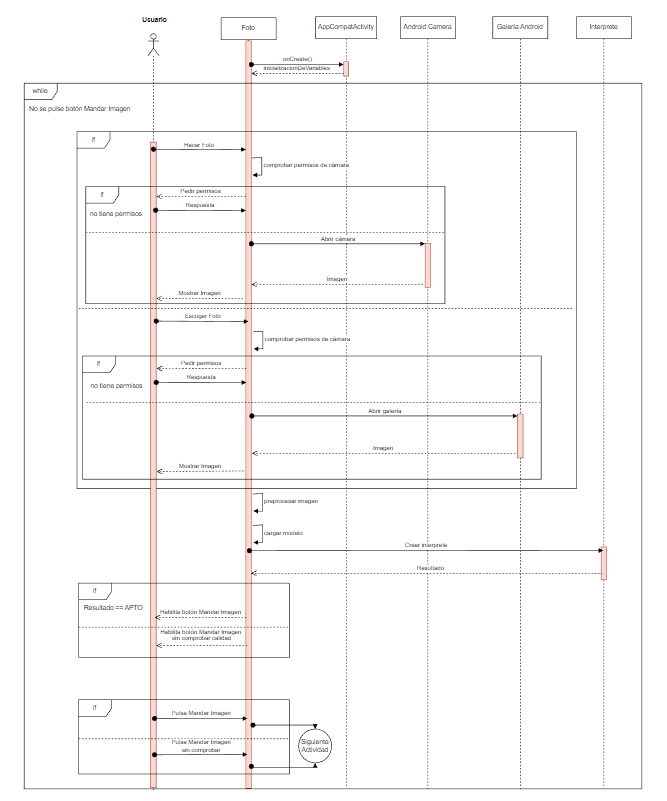
\includegraphics[width=0.9\textwidth]{img/Diagrama de secuencia FOTO.png}
         \caption{Diagrama de secuencia representando a la clase Foto.}
         \label{fig:Diagrama de secuencia Foto}
\end{figure}

En \ref{fig:Diagrama de secuencia RNE}, en este caso, el usuario selecciona las redes neuronales que quiera, y cuando pulsa el botón para crear, se crean tantos hilos como modelos seleccionados, y en el resultado, se calcula la moda, y en caso de empate, la media de ellos. Este resultado, es el que se considera en el expediente, añadiendo los valores al expediente creado y al paciente.

\begin{figure}[!ht]
         \centering
         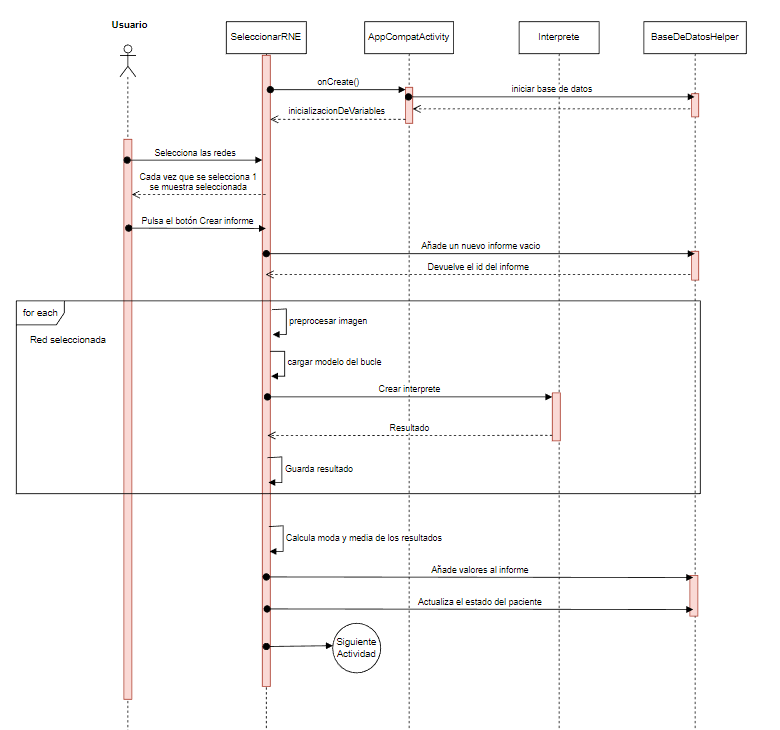
\includegraphics[width=0.9\textwidth]{img/Diagrama de secuencia RNE.png}
         \caption{Diagrama de secuencia representando a la clase SeleccionarRNE.}
         \label{fig:Diagrama de secuencia RNE}
\end{figure}

\section{Diseño arquitectónico}

Como ya se ha explicado en el apartado de ``Técnicas y herramientas'', se ha utilizado un patrón Modelo-Vista-Presentador y un patrón \textit{Singleton}.

\textbf{Modelo-Vista-Presentador}

Es una derivación del patrón modelo-vista-controlador, la diferencia es que se cambia el controlador por un presentador, el cual sirve como intermediario entre el modelo y la interfaz.
        \begin{itemize}
            \item El modelo, define los datos que se utilizan en la interfaz.
            \item El presentador, funciona como intermediario, recuperando los datos del modelo, y cambiando la vista de la interfaz.
            \item La vista, es la interfaz de usuario.
        \end{itemize}
        
        Puesto que Android Studio, ya proporciona separaciones para hacer uso de un modelo-vista-presentador, su implementación ha sido sencilla, donde las \textit{activities} son las diferentes interfaces, los archivos java del directorio ``com.example.retinopatia'' son los presentadores de las vistas, y en el directorio DataBase se encuentra el modelo de datos.

        En la figura \ref{fig:modeloVistaPresentador}, se puede observar su funcionamiento.
        \begin{figure}[!ht]
                 \centering
                 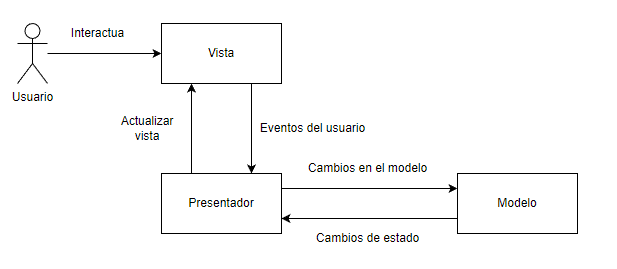
\includegraphics[width=0.9\textwidth]{img/MVP.png}
                  \caption{Modelo-Vista-Presentador}
                 \label{fig:modeloVistaPresentador}
        \end{figure}

        
    \textbf{Patrón singleton}
    
        Este patrón sirve para restringir la creación de objetos. En el caso utilizado, ha sido para la base de datos, de esta forma, no se creaba de cero cada vez que se iniciaba la aplicación.

    \textbf{Diseño de clases}

    Las clases han sido diseñadas todas en el mismo paquete a excepción de la base de datos, la cual debería ser externa a la aplicación y por ello, se ha considerado en otro paquete.

    Cada clase se corresponde con cada una de las vistas del modelo-vista-presentador, estas vistas son las Actividades que se encuentran en el directorio ``res.layout''; a excepción de la clase Utils, la cual es una clase que permite utilidades como abrir un fichero y un switch con los resultados de las imagenes, considerandolo como un convertidor de numero a tipo de retinopatia.

    A continuación se muestran los diagramas de clases resumidos para una mayor comprensión de ellos.
    
    En el primer diagrama de clases, \ref{fig:diagramaClases1}, se puede observar las clases Utils, Foto, Resultados, SelecionarRNE e Interpreter. Como estas incluyen muchas variables y métodos, no se han insertado, exceptuando Utils, que solo incluye 2 métodos estaticos.

    En la figura se puede observar como la clase Foto y SeleccionarRNE hacen uso de la clase Interprete, esto es así, puesto que estas clases son las que integran los modelos. Por otro lado, tanto Foto, como Resultados, como SeleccionarRNE hacen uso de Utils. Foto y SeleccionarRNE hacen uso del método loadFile y SeleccionarRNE y Resultados hacen uso del método SwitchResultados.
    
        \begin{figure}[!ht]
                 \centering
                 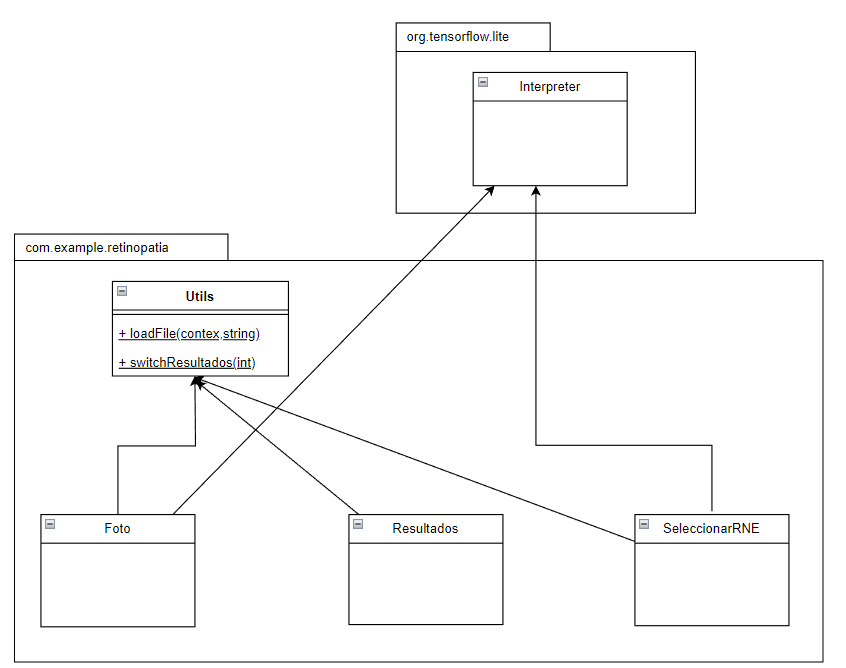
\includegraphics[width=0.9\textwidth]{img/Diagrama de clases 1.png}
                  \caption{Diagrama de clases de Utils e Interprete}
                 \label{fig:diagramaClases1}
        \end{figure}


    En el segundo diagrama de clases, \ref{fig:diagramaClases2}, en el paquete ``com.example.retinopatia'', no se incluyen las clases Foto y Utils. Sabiendo eso, las demas clases importan las clases SQLiteDatabase, Cursor y BaseDeDatosHelper. Por ello, para que no se liasen las líneas, se han introducido estas en los paquetes.

    El motivo de la relación es que la clase BaseDeDatosHelper carga la base de datos sqlite almacenada en el dispositivo, cuando se va a hacer un cambio en esta, se abre en formato lectura o escritura dependiendo de la acción, haciendo uso de la clase SQLiteDatabase.
    Por último, cuando se hace una consulta a la base de datos, es necesario que haya un cursor que recorra las distintas sentencias obtenidas.

            \begin{figure}[!ht]
                 \centering
                 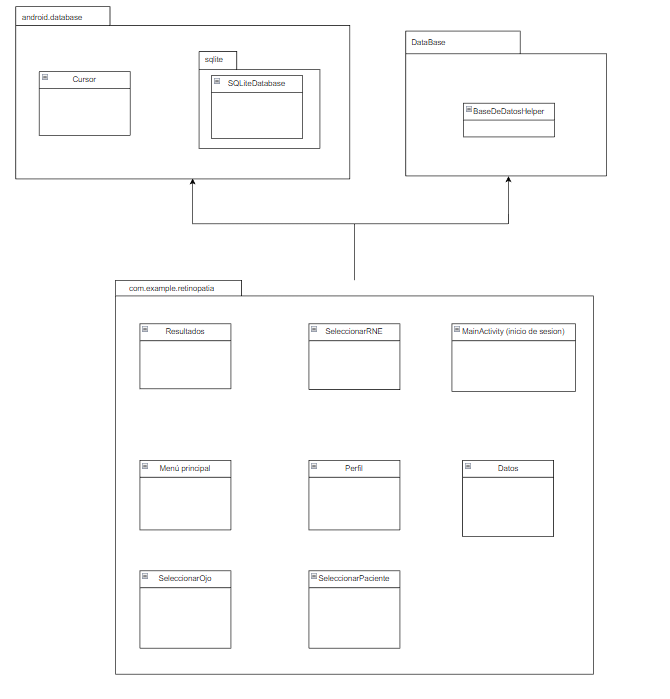
\includegraphics[width=0.9\textwidth]{img/Diagrama de clases 2.png}
                  \caption{Diagrama de clases relativos a la base de datos}
                 \label{fig:diagramaClases2}
        \end{figure}

\section{Diseño de pruebas}

Como se ha comentado, no se han implementado pruebas automáticas, sino pruebas manuales, aun así, se hizo un conjunto de pruebas, para comprobar el funcionamiento de la aplicación.

El conjunto de pruebas se puede ver en las tablas \ref{Pruebas CP-1}, \ref{Pruebas CP-2}, \ref{Pruebas CP-3}, \ref{Pruebas CP-4}


\begin{table}[htbp]
    \centering
    \begin{tabular}{|lc|lc|}
    \toprule
        \textbf{ID de la prueba} & CP1 & \textbf{ID del requisito} & RF-3, RF-3.1 \\
        \textbf{Descripción} & Inicio de sesión & \textbf{Prioridad} & 3 \\

        \textbf{Precondición} &   & \textbf{Postcondición} &   \\
        \bottomrule
    \end{tabular}

    \centering
    \begin{tabular}{clll}
    \toprule
    Paso & Inputs & Resultado esperado & Resultado obtenido  \\
    \midrule
    
    1 & [null,null] & mensaje de error & mensaje de error  \\
    2 & [medico1@gmail.com,null] & mensaje de error & mensaje de error  \\
    3 &[null, contrasena] & mensaje de error & mensaje de error  \\
    4 & [medico1@gmail.com,a] & mensaje de error & mensaje de error \\
    5 & [usuario1@gmail.com,contrasena] & mensaje de error & mensaje de error  \\
    6  & [medico1@gmail.com,contrasena] & inicio de sesión & inicio de sesión  \\
    
    
    \bottomrule
    \end{tabular}
\caption{Pruebas CP-1.}
\label{Pruebas CP-1}
\end{table}


\begin{table}[htbp]
    \centering
    \begin{tabular}{|lc|lc|}
    \toprule
        \textbf{ID de la prueba} & CP2 & \textbf{ID del requisito} & RF-4 \\
        \textbf{Descripción} &  Escoger paciente  & \textbf{Prioridad} & 5\\
        \textbf{Precondición} & Iniciar como médico   & \textbf{Postcondición} &   \\
        \bottomrule
    \end{tabular}

    \centering
    \begin{tabular}{clll}
    \toprule
    Paso & Inputs & Resultado esperado & Resultado obtenido  \\
    \midrule
    
    1 & null & mensaje de error & mensaje de error  \\
    2 & 12345678 & Mensaje paciente1 & mensaje paciente1  \\
    3 & 11111111 & Mensaje médico1 & mensaje médico1  \\
    4 & 12341234 & mensaje de error & mensaje de error \\
    5 & 12345678A & mensaje de error & mensaje de error  \\
    6  & [medico1@gmail.com,contrasena] & inicio de sesión & inicio de sesión  \\
    
    
    \bottomrule
    \end{tabular}
\caption{Pruebas CP-2.}
\label{Pruebas CP-2}
\end{table}

\begin{table}[htbp]
    \centering
    \begin{tabular}{|lc|lc|}
    \toprule
         \textbf{ID de la prueba} & CP3 & \textbf{ID del requisito} & RF-2\\
        \textbf{Descripción} &  Creación y comprobación  & \textbf{Prioridad} & 4\\
            & de los informes invitado & & \\
        \textbf{Precondición} &   & \textbf{Postcondición} &   \\
        \bottomrule
    \end{tabular}
    \centering
    \begin{tabular}{clll}
    \toprule
    Paso & Inputs & Resultado esperado & Resultado obtenido  \\
    \midrule
    
    1 & iniciar sesión como invitado & ir menú principal & ir menú principal  \\
    2 & botón resultados del paciente & 0 informes & 0 informes  \\
    3 & volver & ir menú principal & ir menú principal  \\
    4 & botón sacar foto al paciente & ir menú elegir ojo & ir menú elegir ojo \\
    5 & botón ojo derecho & ir menú sacar foto & ir menú sacar foto  \\
    6  & sacar nueva foto & calidad no es apta & calidad no es apta  \\
    7  & escoger foto no apta & calidad no es apta & calidad no es apta  \\
    8  & escoger foto apta & calidad es apta & calidad es apta  \\
    9  & seleccionar redes y mandar & ir menú elegir ojo & ir menú elegir ojo  \\
    10  & volver & ir menú principal & ir menú principal  \\
    11  & botón resultados del paciente & 1 informe & 1 informe  \\
    
    
    \bottomrule
    \end{tabular}
\caption{Pruebas CP-3.}
\label{Pruebas CP-3}
\end{table}

\begin{table}[htbp]
    \centering
    \begin{tabular}{|lc|lc|}
    \toprule
         \textbf{ID de la prueba} & CP4 & \textbf{ID del requisito} & RF-2\\
        \textbf{Descripción} &  Creación y comprobación  & \textbf{Prioridad} & 5\\
         & de los informes médico & & \\
        \textbf{Precondición} &   & \textbf{Postcondición} &   \\
        \bottomrule
    \end{tabular}
    \centering
    \begin{tabular}{clll}
    \toprule
    Paso & Inputs & Resultado esperado & Resultado obtenido  \\
    \midrule
    
    1 & [medico1@gmail.com,contrasena] & ir seleccionar DNI & ir seleccionar DNI  \\
    2 & 12345678 & ir menú principal & ir menú principal  \\
    2 & botón resultados del paciente & 0 informes & 0 informes  \\
    3 & volver & ir menú principal & ir menú principal  \\
    4 & botón sacar foto al paciente & ir menú elegir ojo & ir menú elegir ojo \\
    5 & botón ojo derecho & ir menú sacar foto & ir menú sacar foto  \\
    6  & sacar nueva foto & calidad no es apta & calidad no es apta  \\
    7  & escoger foto no apta & calidad no es apta & calidad no es apta  \\
    8  & escoger foto apta & calidad es apta & calidad es apta  \\
    9  & seleccionar redes y mandar & ir menú elegir ojo & ir menú elegir ojo  \\
    10  & volver & ir menú principal & ir menú principal  \\
    11  & botón resultados del paciente & 1 informe & 1 informe  \\
    
    
    \bottomrule
    \end{tabular}
\caption{Pruebas CP-4.}
\label{Pruebas CP-4}
\end{table}

\section{Diseño de la aplicación}

Inicialmente se hizo un boceto de como serían las distintas ventanas de la aplicación \ref{fig:interfazInicial}.

        \begin{figure}[!ht]
                 \centering
                 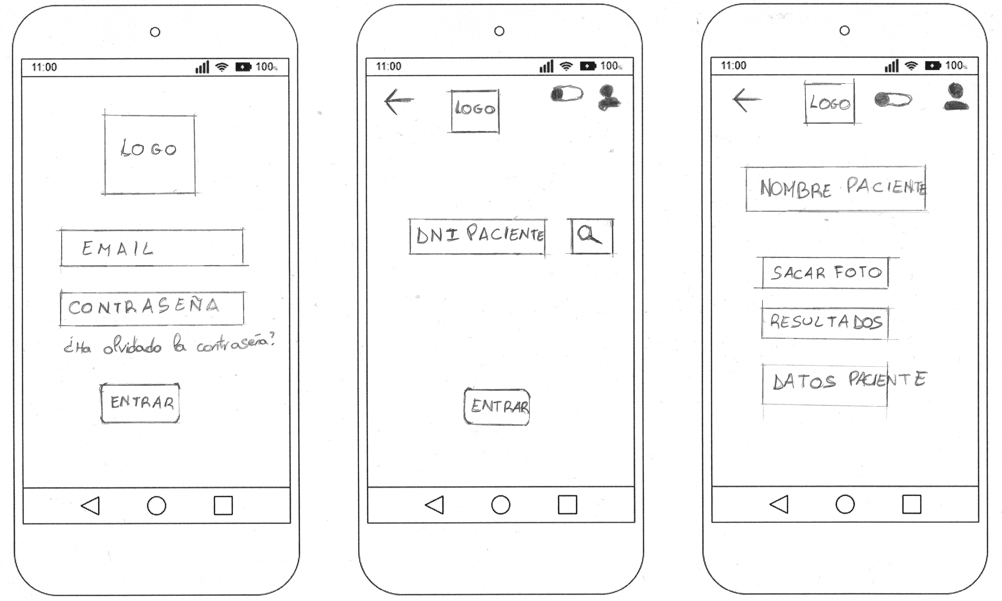
\includegraphics[width=0.6\textwidth]{img/Interfaz1.png}
                 \centering
                 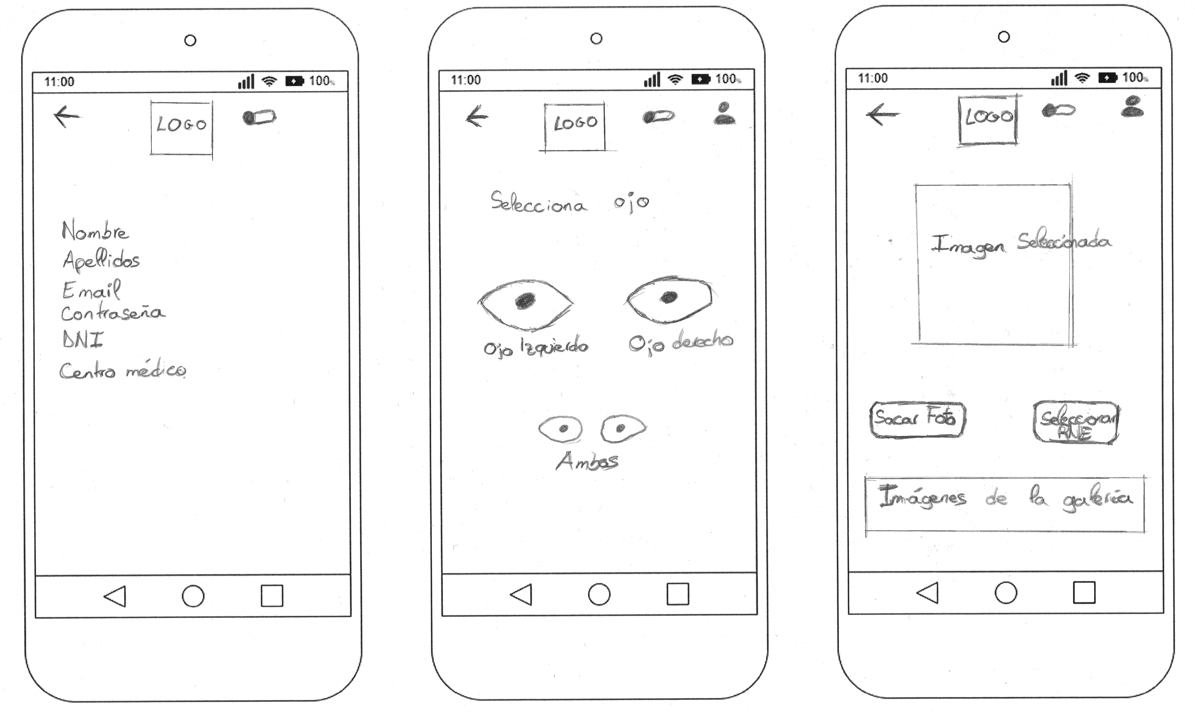
\includegraphics[width=0.6\textwidth]{img/Interfaz2.png}
                 \centering
                 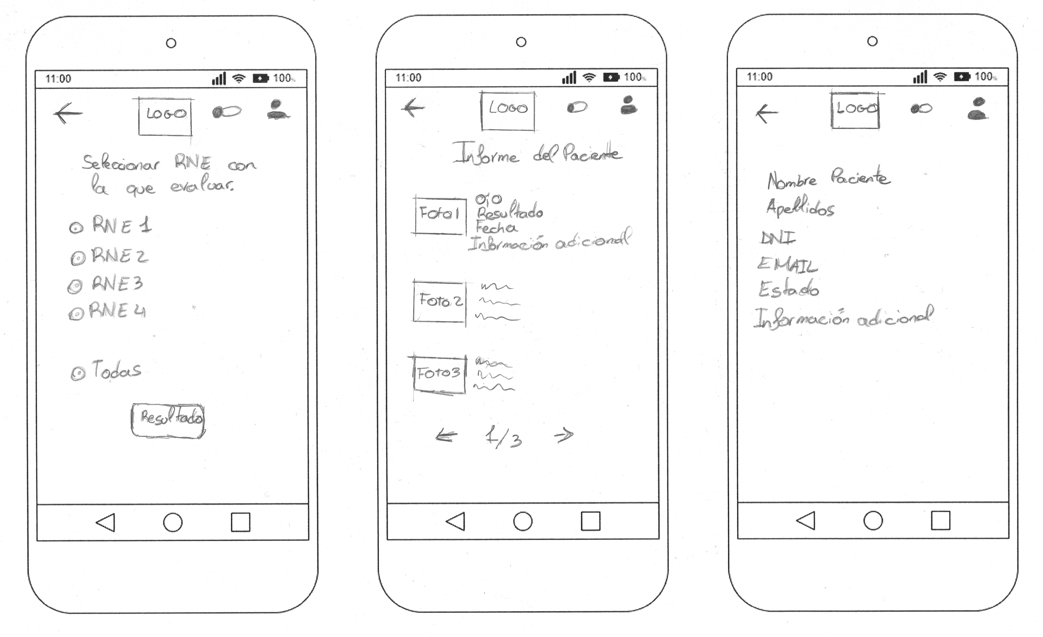
\includegraphics[width=0.6\textwidth]{img/Interfaz3.png}
                  \caption{Interfaz inicial de la aplicación}
                 \label{fig:interfazInicial}
        \end{figure}
        
    Posteriormente, se diseñó el logo de la aplicación, para ello, se utilizó el \textit{prompt} ``Un icono que combine un signo de diabetes con un ojo: esta opción combina el símbolo de la diabetes (un círculo con un punto en el medio) con un ojo para sugerir la relación entre la diabetes y la salud visual. Android app style'' en la herramienta DALL·E, y entre las opciones elegidas, se obtuvo \ref{fig:logoDalle}, y se modificó para obtener \ref{fig:logo}. 

\begin{figure}[!ht]
    \centering
    \begin{minipage}[t]{0.45\textwidth}
        \centering
        
\includegraphics[width=0.385\textwidth]{img/logoDalle.png}
        \caption{Logo obtenido de  Dalle}
        \label{fig:logoDalle}
    \end{minipage}\hfill
    \begin{minipage}[t]{0.45\textwidth}
        \centering
        
\includegraphics[width=0.45\textwidth]{img/logo.png}
        \caption{Logo final}
        \label{fig:logo}
    \end{minipage}
\end{figure}

Y, por último, se diseñó la aplicación final con las interfaces \ref{fig:interfazFinal}

        \begin{figure}[!ht]
                 \centering
                 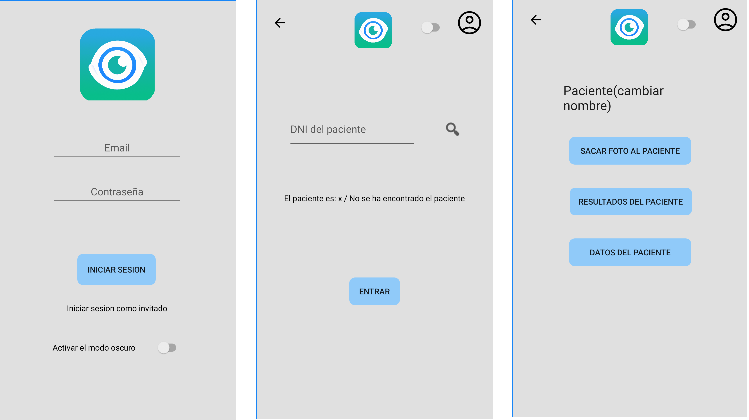
\includegraphics[width=0.6\textwidth]{img/interfaz1-final.png}
                 \centering
                 \includegraphics[width=0.6\textwidth]{img/Interfaz2-final.png}
                 \centering
                 \includegraphics[width=0.6\textwidth]{img/Interfaz3-final.png}
                  \caption{Interfaz final de la aplicación}
                 \label{fig:interfazFinal}
        \end{figure}

La navegación de la aplicación se vería como se puede observar en \ref{fig:diagrama de navegación}
        \begin{figure}[!ht]
                 \centering
                 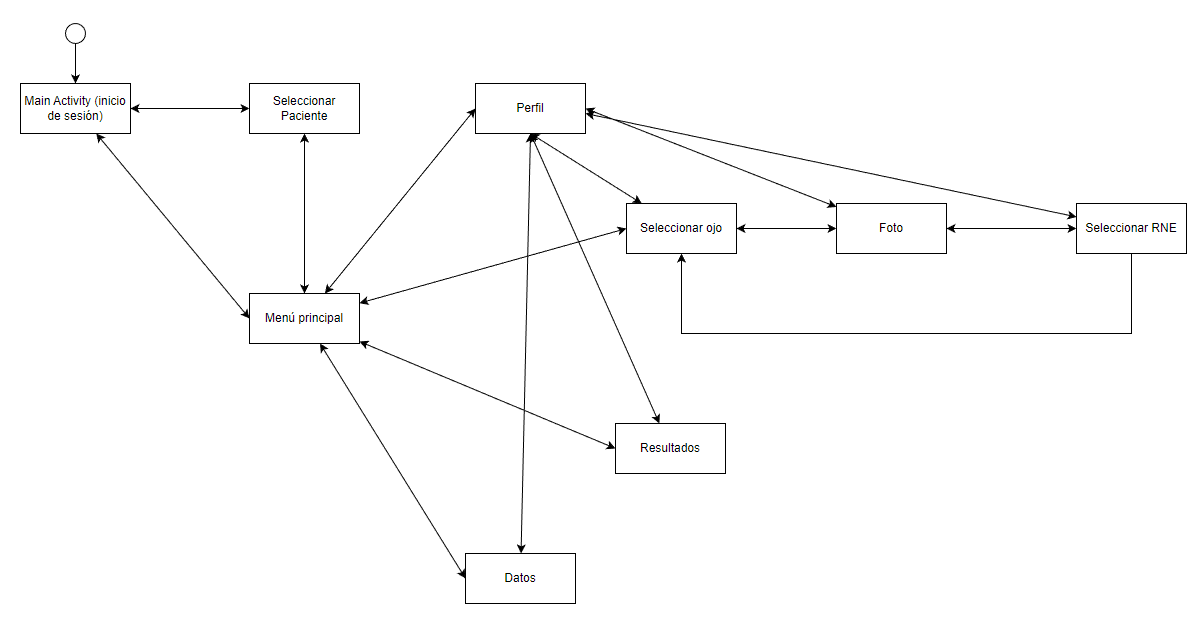
\includegraphics[width=0.6\textwidth]{img/Diagrama de navegacion.png}
                  \caption{Diagrama de navegación de la aplicación}
                 \label{fig:diagrama de navegación}
        \end{figure}